\scanpage{51}
% E: text|upper left, date|2.1.84.
2.1.84.

\deleted{
% E: text|left upper, introduction|On place sur K
On place sur \deleted{\unsure{un graphe}} \(K\) deux ensembles de pts, \(S'_K\ S''_K\) \deleted{\unsure{et}}, de telle façon que
\inserted{\(S'_K\) : sommets rouges ; \(S''_K\) : sommets \unsure{oranges}}

% E: text|left upper, bracketed paragraph|pour toute face
\deleted{\unsure{b)}} \(\forall\ F\) face de \(K\), \(\delta F\cap S'\) est un polygone top. d'ordre \(2n\), et sur chaque côté \inserted{\(\alpha\)} de celui-ci il y a un pt de \(S''\) et un seul, qui est son milieu si \(\alpha\) est \unsure{entier|ordinaire}.

\deleted{a) \(\unsure{S'_K\subset L}\) \unsure{tous les sommets}}
\deleted{a) \(\unsure{S(K)\cap S'_K\supset K\cap L\setminus K\cap S(L)}\)}

% E: display|left middle, a|S'_K intersection L
a) \(S'_K\cap L=K\cap L\setminus(\text{ensemble des pts critiques de }K\text{ qui sont d'ordre impair})\)

\deleted{b) \(S'_K\cap S(K)=S(K)\cap L\)}

% E: text|left middle, b|Pour toute arête
b) \deleted{\unsure{Ensuite}} Pour toute arête (ord.) \(a\) de \(K\), on a \(a\cap S'_K\ne\varnothing\). \inserted{\unsure{des vrais côtés de \(K\),}} et l'unique sommet de \(K\) sur \(\alpha\) dans les cas ci-contre.

% E: drawing|left middle, small crossed segment|green segment red and orange marks
\figure{
\begin{tikzpicture}[scale=.7]
\draw[yellow!60!green,line width=2pt] (0,0)--(2.1,0);
\draw[red!70!black,line width=2pt] (.8,-.13)--(.8,.13) (1.2,-.13)--(1.2,.13);
\draw[orange,line width=3pt] (1,-.12)--(1,.12);
\draw[black,line width=1pt] (-.05,.02)--(.2,.18)--(.06,.08)--(.5,.12)--(.7,.1)--(1.4,.18)--(1.65,.13)--(2.2,.2);
\end{tikzpicture}}

% E: drawing|left middle, lower segment|dotted green segment red centre
\figure{
\begin{tikzpicture}[scale=.8]
\draw[yellow!60!green,line width=2pt,densely dotted] (0,0)--(3.2,.1);
\fill[yellow!60!green] (0,0) circle(.09) (3.2,.1) circle(.09);
\draw[red!70!black,line width=3pt] (1.2,.04)--(2,.07);
\draw[orange,line width=3pt] (1.6,-.17)--(1.6,.27);
\end{tikzpicture}}

% E: drawing|left middle, small angle|green angle orange corner
\figure{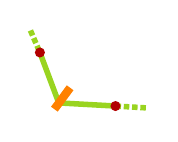
\begin{tikzpicture}[scale=.8]
\draw[yellow!60!green,line width=2pt] (0,1)--(.3,.2)--(1.2,.15);
\draw[yellow!60!green,line width=2pt,densely dotted] (-.15,1.35)--(0,1) (1.2,.15)--(1.7,.12);
\fill[red!70!black] (0,1) circle(.08) (1.2,.15) circle(.08);
\draw[orange,line width=3pt] (.23,.1)--(.48,.44);
\end{tikzpicture}}

% E: text|left lower, NB|a et b impliquent
\uline{NB} a) et b) impliquent que \(S'_K\cap S(K)=S(K)\cap L\), i.e. un sommet de \(K\) est dans \(S'_K\) ssi il est dans \(L\).

% E: text|left bottom, c|Pour tt pt critique
c) Pour tt pt critique \(s\) de \(K\), sur l'arête
\deleted{\(S'_K\setminus S_K\cap L\) est réunion de segments, \unsure{en plus de quelques pts isolés de \(K\) qui}}
désignons par \(t',t''\) les pts les plus proches de \(s\), sur l'arête \(a\) de \(K\) contenant \(s\), parmi les pts de \((a\cap L)\unsure{\cap|\cup}\partial a\).
L'intersection \([t',t'']\cap S'_K\) est de cardinal égal :
\deleted{\unsure{on disposera sur le segment \([t',t'']\)}}
\(\nu(s)\), \deleted{et il y a \unsure{un}}
}

% E: drawing|right top|oval thick boundary arcs crossing curves
\figure{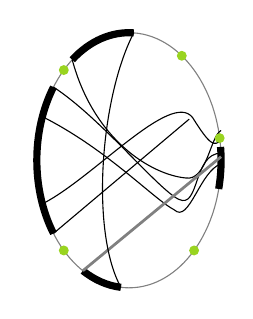
\begin{tikzpicture}[x=1cm,y=1cm,scale=.9]
\draw[gray] (0,0) ellipse (1.3 and 1.8);
\draw[line width=2.6pt] (87:1.3 and 1.8) arc(87:128:1.3 and 1.8) (145:1.3 and 1.8) arc(145:215:1.3 and 1.8) (240:1.3 and 1.8) arc(240:265:1.3 and 1.8) (-13:1.3 and 1.8) arc(-13:6:1.3 and 1.8);
\draw (145:1.3 and 1.8) .. controls (-.4,.6) and (.4,-.4) .. (.7,-.55) .. controls (1,-.7) and (.9,.1) .. (1.3,.1);
\draw (128:1.3 and 1.8) .. controls (-.5,.3) and (.3,-.2) .. (.8,-.25) .. controls (1.1,-.3) and (1.15,.35) .. (1.3,.42);
\draw (160:1.3 and 1.8) .. controls (-.3,.15) and (.35,-.55) .. (.64,-.7) .. controls (.85,-.9) and (1,-.15) .. (1.3,-.05);
\draw (200:1.3 and 1.8) .. controls (-.5,-.25) and (.6,1) .. (.9,.6) .. controls (1.15,.2) and (1.2,.2) .. (1.3,.28);
\draw (215:1.3 and 1.8)--(.85,.58);
\draw[gray,line width=1pt] (240:1.3 and 1.8)--(1.3,.05);
\draw (265:1.3 and 1.8) .. controls (-.55,-1) and (-.4,.9) .. (87:1.3 and 1.8);
\foreach \a in {135,55,10,225,315}{\fill[yellow!60!green] (\a:1.3 and 1.8) circle(.07);}
\end{tikzpicture}}

% E: drawing|right middle left|red hexagon central orange point green arrows
\figure{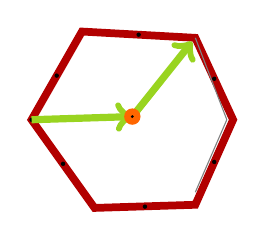
\begin{tikzpicture}[scale=.8]
\draw[red!70!black,line width=2.8pt] (0,1.5)--(.8,2.9)--(2.6,2.8)--(3.2,1.5)--(2.6,.15)--(1,.1)--cycle;
\foreach \p in {(0,1.5),(.4,2.2),(1.7,2.85),(2.9,2.15),(2.9,.83),(1.8,.12),(.5,.8)}{\fill \p circle(.035);}
\draw[yellow!60!green,line width=2.6pt,->] (0,1.5)--(1.6,1.55);
\draw[yellow!60!green,line width=2.6pt,->] (1.6,1.55)--(2.55,2.74);
\fill[orange!80!red] (1.6,1.55) circle(.13);
\fill[black] (1.6,1.55) circle(.025);
\draw[gray] (2.6,2.8)--(3.1,1.5)--(2.6,.35);
\end{tikzpicture}}

% E: drawing|right middle right|red pentagon green straight passage
\figure{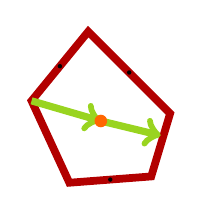
\begin{tikzpicture}[scale=.8]
\draw[red!70!black,line width=2.8pt] (0,1.3)--(.9,2.4)--(2.2,1.1)--(1.9,.1)--(.6,0)--cycle;
\foreach \p in {(.45,1.85),(1.55,1.75),(1.25,.05)}{\fill \p circle(.035);}
\draw[yellow!60!green,line width=2.6pt,->] (0,1.3)--(1.1,.98);
\draw[yellow!60!green,line width=2.6pt,->] (1.1,.98)--(2.05,.75);
\fill[orange!80!red] (1.1,.98) circle(.1);
\end{tikzpicture}}

% E: drawing|right lower middle|broken red polygon green bent arrows pencil lines
\figure{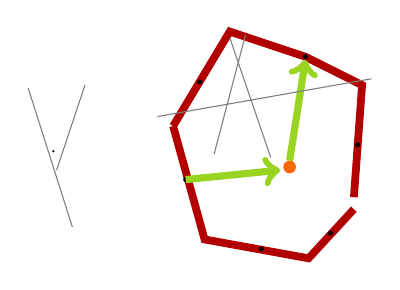
\begin{tikzpicture}[scale=.8]
\draw[red!70!black,line width=2.8pt] (0,1.8)--(.9,3.3)--(2.1,2.9)--(3,2.45)--(2.87,.67) (2.87,.48)--(2.15,-.3)--(.5,0)--(0,1.8);
\foreach \p in {(.42,2.5),(2.1,2.9),(2.93,1.5),(2.5,.1),(1.4,-.15),(.2,.95)}{\fill \p circle(.04);}
\draw[yellow!60!green,line width=2.6pt,->] (.2,.95)--(1.7,1.1);
\draw[yellow!60!green,line width=2.6pt,->] (1.85,1.25)--(2.1,2.85);
\fill[orange!80!red] (1.85,1.15) circle(.1);
\draw[gray] (-.25,1.95)--(3.15,2.55) (.9,3.2)--(1.55,1.3) (1.15,3.25)--(.65,1.35);
\draw[gray] (-2.3,2.4)--(-1.6,.2) (-1.4,2.45)--(-1.85,1.1);
\fill (-1.9,1.4) circle(.02);
\end{tikzpicture}}

% E: drawing|right bottom right|three red crossing branches green passage
\figure{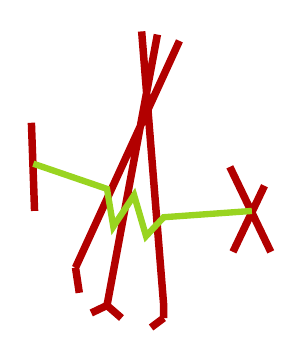
\begin{tikzpicture}[scale=.8]
\draw[red!70!black,line width=2.7pt] (0,.6)--(1.65,4.2) (0,.6)--(.06,.2) (.5,0)--(1.3,4.3) (.25,-.12)--(.5,0)--(.73,-.2) (1.4,-.2)--(1.4,0)--(1.05,4.35) (1.4,-.2)--(1.2,-.35) (-.65,1.5)--(-.7,2.9) (2.5,.85)--(3,1.9) (2.45,2.2)--(3.1,.85);
\draw[yellow!60!green,line width=2.3pt] (-.67,2.25)--(.5,1.85)--(.6,1.25)--(.93,1.75)--(1.12,1.1)--(1.4,1.4)--(2.8,1.5);
\end{tikzpicture}}

% E: drawing|right bottom left|red crossing graph green W and dotted segments
\figure{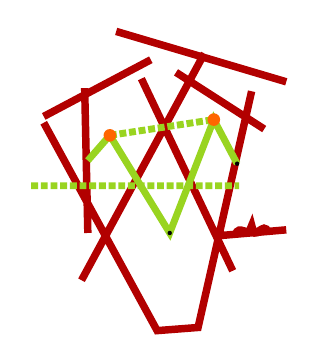
\begin{tikzpicture}[scale=.8]
\draw[red!70!black,line width=2.7pt] (0,3)--(1.8,-.3)--(2.45,-.25)--(3.3,3.5) (.6,.5)--(2.55,4.1) (.7,1.25)--(.65,3.55) (1.55,3.7)--(3,0.65) (0,3.1)--(1.7,4) (1.15,4.45)--(3.85,3.65) (2.1,3.8)--(3.5,2.9) (2.7,1.2)--(3.85,1.3);
\draw[yellow!60!green,line width=2.5pt] (.7,2.4)--(1.05,2.8)--(2,1.25)--(2.7,3.05)--(3.07,2.35);
\draw[yellow!60!green,line width=2.5pt,densely dotted] (1.05,2.8)--(2.7,3.05) (-.2,2)--(3.1,2);
\fill[orange!80!red] (1.05,2.8) circle(.1) (2.7,3.05) circle(.1);
\fill (2,1.25) circle(.035) (3.07,2.35) circle(.035);
\draw[red!70!black,line width=3pt] (3.05,1.22)..controls (3.1,1.4) and (3.25,1.15)..(3.3,1.35)..controls (3.35,1.1) and (3.5,1.45)..(3.55,1.26);
\end{tikzpicture}}
\mspage{50}
